% Diese Zeile bitte -nicht- aendern.
\documentclass[course=asp]{aspdoc}

%newly added packages
\usepackage{microtype}
\usepackage{graphicx}
\usepackage{wrapfig}
\usepackage{enumitem}
\usepackage{amssymb}
\usepackage{amsthm}
\usepackage{listings}

\usepackage{amsmath}	%eins von beidem?
\usepackage{mathtools}

\usepackage{index}

%%%%%%%%%%%%%%%%%%%%%%%%%%%%%%%%%
%% TODO: Ersetzen Sie in den folgenden Zeilen die entsprechenden -Texte-
%% mit den richtigen Werten.
\newcommand{\theGroup}{132} % Beispiel: 42
\newcommand{\theNumber}{A214} % Beispiel: A123
\author{Mohammed Attia \and Patrick Zimmermann \and Thomas Torggler}
\date{Wintersemester 2020/21} % Beispiel: Wintersemester 2019/20
%%%%%%%%%%%%%%%%%%%%%%%%%%%%%%%%%

% Diese Zeile bitte -nicht- aendern.
\title{Gruppe \theGroup{} -- Abgabe zu Aufgabe \theNumber}

\begin{document}
\maketitle

\newpage
\section{Einleitung}

Raumf\"ullende Kurven bilden eine Br\"ucke zwischen Kunst und mathematischer Geometrie. In der Mathematik werden sie gemeinhin benutzt um ein $n$-dimensionales Problem in ein Eindimensionales zu konvertieren. Eine solche Kurve beschreibt grunds\"atzlich einen linearen Pfad durch $n$-dimensionale R\"aume. Giuseppe Peano war der Erste, der eine solche Kurve 1890 definierte.

Um einen n-dimensionalen Raum in die Dimension n-1 zu konvertieren, l\"asst sich eine stetig surrjektive Funktion $f(x)$ erstellen, so dass gilt: $\forall x \in \mathbb{R}^{n-1} \quad \exists y \in \mathbb{R}^n$. F\"ur einen Beweis siehe (QUELLE?). Hier wollen wir uns auf die sogenannten Peano-Kurven beschr\"anken. F\"ur eine solche Kurve definieren wir ein Intervall $I = [0;1]$, sowie  $f: I \rightarrow I^2 $. Dann ist die Peano-Kurve: $\lim\limits_{x \to \infty}f(x)$, mit $x \in I$. Sie \{ entspricht dem Grenzwert einer Folge von Funktionen f(x) und \} l\"asst sich mit der Bedingung, dass sich die Kurve nicht \"uberschneiden darf, folgendermaßen konstruieren:

Man unterteile eine Fl\"ache in 9 Quadrate. Jedes dieser Quadrate soll nun durch eine Kurve durchlaufen werden. Dadurch durchl\"auft die Kurve die Quadrate in Form eines „S“.
In einem Iterationsschritt l\"asst sich eines der 9 Quadrate in weitere 9 Quadrate Unterteilen, die wiederum auf dieselbe Art verbunden werden, wie in Abb.1 gezeigt.

\begin{figure} [ht] %vorher, eigentlich bild unter text
\centering
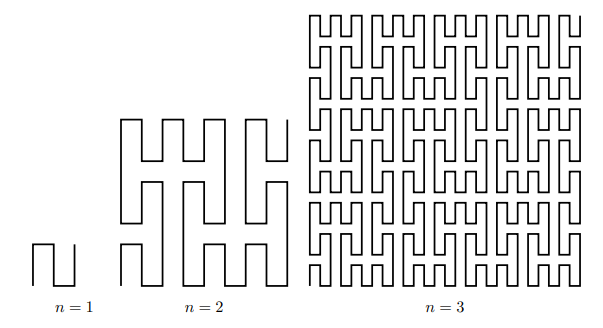
\includegraphics[scale=0.9]{PeanoBsp.png}
\caption{Peano-Kurve mit n = \{1, 2, 3\}, ~\cite{aufgabenstellung}}\label{Abb:Peano}	
\end{figure}

Im Folgenden definieren wir $n \in \mathbb{N}$ als Grad der Kurve.
Wir beschreiben nun unseren Ansatz, einen iterativen Algorithmus mit dem Grad $n$ als Eingabe zu finden, um die eben beschriebene Peano-Kurve darzustellen. Die hierbei generierten Punkte werden in ihrer Reihenfolge ausgegeben. Anders als in der beschriebenen mathematischen Definition werden wir jedoch nicht nur nach $[0;1]$, sondern nach $\mathbb{N}$ abbilden.

%Ergebnis hier einf\"ugen!! dann ist auch das Format besser

\newpage

\section{L\"osungsansatz}

\subsection{Algorithmus}

Der Aufbau der Peano-Kurve erm\"oglicht es, die Kurve des aktuellen Grades mit einer Variation der originalen Kurve des vorherigen Grades und deren Permutationen zu zeichnen. Wie in Abbildung 2 gezeigt gibt es ingesamt drei Permutationen der Kurve:

\begin{itemize}
    \item Die Invertierung, bei der jeder Schritt in seinen entsprechenden Gegenschritt ge\"andert wird.
    \item Die Spiegelung, bei der nur die vertikalen Schritte ge\"andert werden.
    \item Die gespiegelte Invertierung, bei der beide der vorherigen Permutationen vorgenommen werden.
\end{itemize}

Diese Observation war der Grundstein unseres iterativen Algorithmus. Anfangs wird dabei die Startkurve hardcodiert in einem Integerarray mit Interval $[0;3]$ abgespeichert. Die Zahlen stehen dabei jeweils f\"ur eine der vier Richtungen: 0 f\"ur oben, 1 f\"ur rechts, 2 f\"ur unten und 3 f\"ur links. Beispielsweise sieht also die orignale Kurve des ersten Grades wie folgt aus $\{0, 0, 1, 2, 2, 1, 0, 0\}$ und die dazugeh\"orige Invertierung ist $\{2, 2, 3, 0, 0, 3, 2, 2\}$. 
Falls der eingegebene Grad $n > 1$ ist, wird startend vom Grad 2 aufsteigend \"uber alle Grade $m$ bis inklusive $n$ iteriert. Bei jeder Iteration wird abwechselnd ein Verbindungschritt hardcodiert in den Array geschrieben und danach die entsprechende Permutation der Kurve des vorherigen Grades $m - 1$ berechnet und eingef\"ugt. Dieser Schritt wird f\"ur die acht fehlenden Teilkurven des aktuellen Grades $m$ ausgef\"uhrt, sodass Schritt f\"ur Schritt die vollst\"andige Kurve entsteht.

\begin{figure}[ht]
\centering
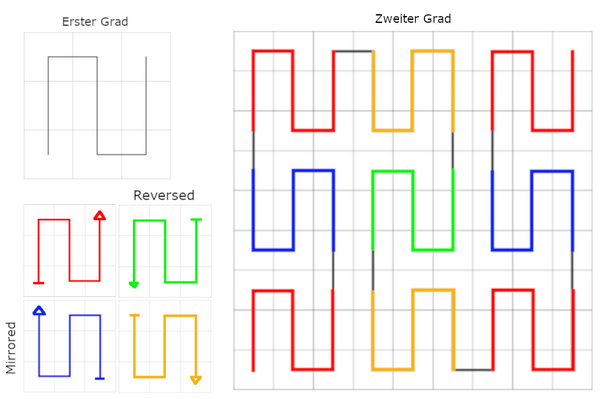
\includegraphics[scale=0.32]{PeanoFarbcodiert.png}
\caption{Peano-Kurve mit n = 1, n = 2}\label{Abb:Peano L\"osungsidee}
\end{figure}

Nachdem \"uber alle Grade iteriert wurde oder der eingegebene Grad $n = 1$ ist, l\"auft der Algorithmus den vollst\"andigen Richtungs-Array durch, ver\"andert dabei bei jedem Schritt je nach Richtungsangabe entweder die x oder y-Koordinate und speichert diese dann in die Ausgabeliste der Peano-Methode.

\subsection{Umgesetzte Optimierungen}

Im urspr\"unglichen Entwurf des Algorithmus wurden die drei verschiedenen Permutationen vor jeder Iteration einmal berechnet und als einzelne Arrays abgespeichert um sie danach wenn sie ben\"otigt werden nur mehr an die jeweiligen Stellen in den gro\ss en Richtungsarray zu kopieren. Da dadurch jedoch ein erh\"ohter Speicheraufwand entsteht haben wir uns daf\"ur entschieden jede Permutation immer neu zu berechnen, wenn sie gebraucht wird und diese direkt in den Array zu speichern. Dies schien f\"ur uns ein sinnvoller Optimierungsansatz zu sein, da jede Permutation wie in Abbildung 2 zu sehen maximal zweimal vorkommt. Allein die Originalkurve wird dreimal ben\"otigt und auf diese kann immer sehr schnell zugegriffen werden, indem man auf die Werte an den Adressen von $0$ bis $9^{(m - 1)} - 2$ im Richtungsarray zugreift. 

% Ein calleesaved register weniger verwendet

\subsection{Alternativer L\"osungsansatz}

Wir haben uns bewusst gegen die Nutzung von SIMD-Befehlen entschieden, da der einzige Anwendungspunkt die synchrone Umrechnung der Richtungen in den Permutationsmethoden zu den Koordinaten w\"are. Da wir 64-Bit gro\ss e Koordinatenstellen benutzen, k\"onnen wir maximal zwei Koordinaten gleichzeitig verrechnen. Hinzu kommt, dass die Peano-Kurve mit der hier beschriebenen Berechnung maximal zwei Richtungen hintereinander verrechnen kann, da die Kurve danach die Richtung \"andert und man nicht mehr die selbe Berechnung parallel ausf\"uhren kann.

So w\"urde sich der Algorithmus in einem alternativen L\"osungsansatz noch zus\"atzlich optimieren lassen.  

Alternativ haben wir gegen Ende der Bearbeitungszeit eine M\"oglichkeit gefunden den Richtungsarray auszulassen und die gesamte Koordinatenberechnung direkt durchzuf\"uhren. Dies w\"urde nat\"urlich sehr viel Rechen- und Speicheraufwand einsparen und damit ingesamt bessere Performanzergebnisse erzielen.

\newpage

\section{Korrektheit} % oder Genauigkeit

% Beweisen, dass nichts anderes als die gew\"unschten Permutationen entstehen!!
%TODO: Kapitel Technische Limitationen hier einfuegen! - Die Vorgehensweise ist wissenschaftlich zu dokumentieren. Insbesondere sollten
%angemessene Vergleiche und Eingabebereiche gewaehlt und begruendet werden

Die Genauigkeit unseres Algorithmus ist abh\"angig von dem Grad $n$, das die Anzahl an Iterationen bestimmt, wie in den Abb.1 beschrieben. Das geht auch aus der beschriebenen mathematischen Definition hervor, da die Peano-Kurve an sich ein Grenzwert ist. Somit wird der Algorithmus pr\"aziser, je gr\"o\ss er der Grad der Kurve ist, da die Punkte auf der Kurve sich ebenfalls einem Grenzwert ann\"ahern. Ansonsten ist die Kurve wie oben beschrieben, definiert, weshalb nun die Korrektheit unseres Algorithmus entscheidend ist.
Grunds\"atzlich l\"asst sich die Korrektheit einer Kurve, besonders bei der von uns behandelten, nachweisen, indem man ihre graphischen Darstellungen vergleicht. Da das theoretisch aber nicht m\"oglich ist, folgt auch eine Implementierung in Assambler und in C, die wir auch hinsichtlich ihrer Performanz analysieren wollen.
Dennoch soll der bereits beschriebene Ansatz auf Korrektheit gepr\"uft werden.


Da die eigentliche Koordinatenberechnung abh\"angig von der zuvor ermittelten Richtung ist, ist der folgende Beweis prim\"ar auf die Berechnung der Richtungen ausgerichtet.
Die Koordinatenberechnung findet anschlie\ss end und basierend auf den bisherigen Ergebnissen statt, indem ab\"angig von der Richtung jeweils die X- und die Y-Koordinate eines Z\"ahlers inkrementiert (oder dekrementiert) und abgespeichert wird.

\subsection{Beweis der Permutationen durch Induktion}
Nachdem die Kurve immer wieder die gleichen, teilweise elementaren, Bestandteile verwendet m\"ussen diese und deren Permutationen richtig berechnet werden. Im Speziellen sind das die Kurven mit $n = 1$ und $n = 2$. Aus diesen l\"asst sich induktiv die Korrektheit beweisen, da wir, wie im vorherigen Kapitel beschrieben, zum Berechnen einer Kurve $n$-ten Grades nur die Kurve des Grads $n - 1$ sowie die gespiegelte und invertierte Version dieser Kurve benutzen. Bei der als invertierten Version betitelten Permutation handelt es sich in diesem Kontext um eine Punktspiegelung im Mittelpunkt der vorhergehenden Kurve, siehe Abb.2, weitere Erl\"auterungen folgen.	%echt Punktsymetrisch?

\subsubsection{Induktionsbasis}
Beginnen wir mit $n = 1$. Hier ist die Kurve vordefiniert, dementsprechend gibt es nichts zu zeigen. Da auf diesem Muster alle anderen Kurven mit $n > 1$ basieren, ist sie in unserem Algorithmus ebenfalls als Basis vorgegeben.
Des Weiteren ist die Definition der Kurve mit $n = 2$ f\"ur die Berechnung aller weiteren Kurven n\"otig, da man anhand dieser Kurve alle notwendigen Bedingungen der Konstruktion weiterer Kurven ableiten kann. Deshalb nehmen wir sie also auch als definiert an \cite{aufgabenstellung}. Diese Bedingungen sollen im folgenden ebenfalls gepr\"uft werden.

\subsubsection{Induktionsannahme}
Da die Funktion wie vorher definiert surrjektiv ist, gilt:

\begin{center}
$\forall n > 1 \in \mathbb{N}$, $\exists y \in \mathbb{R}^n$ mit $x \in [0,1]$: $f(x)= y$	%evtl \"andern...
\end{center}

Dadurch lassen sich Kurven mit h\"oherem Grad konstruieren. Es sei nun $n > 1$ und $n$ beliebig gew\"ahlt.

\subsubsection{Induktionsschritt}
Betrachten wir nun Kurven $n$-ten Grades. Hierzu m\"ussen wir die Permutationen der vorhergehenden Kurve untersuchen, die wir zur Konstruktion der Kurve mit Grad n ben\"otigen.
%natuerlich nur, wenn  wir unseren Algorithm behalten
Da diese Permutationen stets auf \"ahnliche Art konstruiert werden, n\"amlich durch Addition von 2 zu der gespeicherten Richtung mit anschlie\ss endem \textit{modulo} 4, um die Richtung wieder in den g\"ultigen Bereich abzubilden. Dadurch ist gewehrleistet, dass durch Mehrfachanwendung einer Funktion, die eine solche Permutation generiert, immer nur die Orginale Kurve oder die gew\"unschte Permutation entstehen kann. Dies wird durch den Wertebereich von $[0;3]$ und der \textit{modulo} 4 erreicht, da so die geraden Werte auf den jeweils anderen geraden Wert abgebildet werden, f\"ur die ungerade Zahlen analog. Dieser Umstand wird bei dem Erstellen der Permutationen ausgenutzt.
Da die Funktionen, die die Permutationen erz\"augen, auf die ganze Kurve des Grades $n = n - 1$ angewand wird, ist sicher gestellt, dass die Permutationen keine anderweitigen Fehler in der Richtgsberechnung besitzten.

\textbf{Die Permutationen:}% - Reverse in Implementierung

Die invertierte Permutation ist im Kern nichts anderes als die normale Peano-Kurve mit anderer Reihenfolge der Koordinatenberechnung, im Speziellen von $p_1=(1,1)$ nach $p_2 = (0,0)$. Dies hat zur Folge, dass sich au\ss er der invertierten Reihenfolge der Punkte an der grundlegenden Kurve nichts \"andert. Somit ist die invertierte Permutation induktiv eben so korrekt wie die zugrundeliegende Kurve niedrigeren Grades, siehe auch Abb.2, gr\"une Kurve.

%\textbf{Spiegelung:}% - Mirror in Implementierung
Bei der Spiegelung wird die Kurve an der X-Achse gespiegelt. Wir ver\"andern also ebenfalls die vertikale Richtung, behalten jedoch weiterhin die horizontale Richtung bei. Dadurch wird die vorausgehende Kurve notwendigerweise abge\"andert. Diese zus\"atzliche Operation ist elementar und greift auf die gespeicherte Richtung einer Koordinate direkt zu. Somit hat diese Opertaion nur indirekt auf die Koordinatenberechnung Einfluss, ohne die Kurve anderweitig zu ver\"andern. Siehe auch Abb.2, gelbe Kurve. %wirklich elementar

%\textbf{Kombination Beider Permutationen:}
Abschlie\ss end bleibt noch die Kombination aus den vorangehenden Permutationen, die ebenfalls f\"ur die Konstruktion der Kurve notwendig ist. Diese Permutation ist, \"ahnlich zu der vorherigen Permutation, eine Spiegelung an der Y-Achse. Dabei wird die horizontale Richtung gewechselt und die Vertikale beibehalten. Ansonsten verh\"alt es sich analog zur Spiegelung.
Siehe auch hier Abb.2, blaue Kurve.

\textbf{Verbinden der Permutationen:}

Die unterschiedlichen Permutationen der Peano-Kurve werden durch eine ebensolche Kurve mit $n = 1$ verbunden. Dadurch bleiben alle Eigenschaften der Kurve erhalten, da wir keine weiteren Punkte in die Kurve einf\"ugen, sondern nur die Art der graphischen Darstellung. Wir f\"ugen also einen weiteren hardcodiertern Schritt zu den bisherigen Richtungen hinzu, um die Koordinaten sp\"ater korrekt zu berechn. Dies ist zudem Teil der Definition dieser Kurve.  


\subsection{Technische Limitationen} %in C
Bei dem Testen unseres Programms fallen bei Graden von $n > 6$ bestimmte technische Limitationen unser Rechensysteme auf. 

Zum einen haben wir kein Programm gefunden, dass die generierten .svg Dateien von einer Gr\"o\ss e 43.0 Megabyte (Peano-Kurve mit $n = 7$) \"offnen kann. Mit zunehmendem Grad enth\"alt die .svg Datei logischerweise immer mehr Punkte der Kurve, weshalb die Gr\"o\ss e ebenfalls exponentiell zur Basis 9 steigt. Deshalb m\"ochten wir an dieser Stelle auf das Kapitel \textit{Korrektheit} verweisen, um die Kurve auf selbige zu pr\"ufen.  %selbige gross?

Zum anderen ist es nicht m\"oglich, beliebig viel Speicher zu allokieren, da die von uns benutzte \textit{malloc}-Funktion maximal 17.179.869.184 Bytes auf dem Heap unser Testumgebungen allokieren kann und der Heap zus\"atzlich in seiner Gr\"o\ss e auf Seite der Hardware begrenzt ist. Deshalb k\"onnen wir auf unseren Systemen die Funktion mit maximal $n = 9$ ausf\"uhren, da sonst nicht gen\"ugend Speicher allokiert wird. F\"ur $n = 10$ m\"ussten 27.894.275.208 Bytes allokiert werden, wozu wir eben nicht im Stande sind. 

Um zu ermitteln, wie viel Speicher wir allokieren k\"onnen, haben wir eine For-Schleife  folgenden Typs ausgef\"uhrt:

\begin{lstlisting} %Formatieren! 

u_int64_t *v;
for (u_int64_t i = 1; v = (u_int64_t *) malloc(i); i <<= 1)   
{     
    print(i); free(v);
}
\end{lstlisting}

Zus\"atzlich evaluierte ein Test, der \"uberpr\"uft, ob der von \textit{malloc} zur\"uckgegebenen Pointer (bei einem $n > 9$) NULL ist, auf unseren Testplatformen ausnahmslos \textit{true}. % also war NUll

Deshalb ist der Wertebereich von $n$ in den Tests im nachfolgenden Kapitel auf $ n \in [1;9]$ limitiert.

Als ein Beispiel f\"ur diesen Algortihmus sei auf Abb.3 verwiesen, welche die erstellte Kurve mit $n = 4$ zeigt. F\"ur ein $n < 4$ werden Bilder erzeugt, die den Kurven in Abb.1 entsprechen. F\"ur $n > 4$ ist die Kurve aufgrund der hohen Dichte in diesem Dokument schwer lesbar darstellbar.

%TODO: Bild mit grad 4 einfuegen, Relevante Beispiele angeben, die die Funktionalit�t und Korrektheit demonstrieren und eventuelle Aussagen unterst�tzen

%TODO: Mathematischen sachen be/ver-weisen!

\newpage
\section{Performanzanalyse}
Bevor wir den bereits ausgef\"uhrten Algorithmus hinsichtlich seiner Performanz analysieren, beschreiben wir kurz die Algorithmen, die wir zu den Vergleichen heranziehen.

Als erstes implemenierten wir den bereits erl\"auterten Algorithmus aus dem Kapitel  \textit{L\"osungsansatz} in C. Um die Performanz-Unterschiede zwischen der direkten Berechnung, im Weiteren als Inplace-Variante, und der einmaligen Berechnung und Speicherung der Permutationen, im Folgenden als Out-Of-Place-Variante bezeichnet, zu analysieren erweitern wir die Implementation um einen entsprechenden Algorithmus, welcher eine abgewandelte Form der Inplace-Variante ist. Der Unterschied besteht darin, dass sobald wir eine Kurve mit $n > 2$ berechnen, speichern wir die schon vorher besprochenen Permutationen der Kurve mit Grad $n - 1$.


%Assembler

\newpage
\section{Zusammenfassung und Ausblick}

%Idee am ende, keine Zeit zur Umsetztung
%statt inplace direkt Koordinatenberechnung

%Hilbert vs Peano


\newpage
% TODO: Fuegen Sie Ihre Quellen der Datei Ausarbeitung.bib hinzu			!!!!
% Referenzieren Sie diese dann mit \cite{}.
% Beispiel: CR2 ist ein Register der x86-Architektur~\cite{intel2017man}.
\bibliographystyle{plain}
\bibliography{Ausarbeitung}{}

\end{document}
